% Created 2024-10-17 Thu 22:52
% Intended LaTeX compiler: pdflatex
\documentclass[11pt]{article}
\usepackage[utf8]{inputenc}
\usepackage[T1]{fontenc}
\usepackage{graphicx}
\usepackage{longtable}
\usepackage{wrapfig}
\usepackage{rotating}
\usepackage[normalem]{ulem}
\usepackage{amsmath}
\usepackage{amssymb}
\usepackage{capt-of}
\usepackage{hyperref}
\usepackage{parskip,darkmode}
\enabledarkmode
\usepackage{tikz}
\usetikzlibrary{positioning, calc}
\author{Arnav Gupta}
\date{\today}
\title{States And Uninformed Search}
\hypersetup{
 pdfauthor={Arnav Gupta},
 pdftitle={States And Uninformed Search},
 pdfkeywords={},
 pdfsubject={},
 pdfcreator={Emacs 29.4 (Org mode 9.7.11)}, 
 pdflang={English}}
\begin{document}

\maketitle
\tableofcontents

\section{Introduction to Search}
\label{sec:org4afc4ee}
Solving some problems requires searching for a solution by searching a directed graph that is
the \textbf{state space} of the problem.
A graph consists of a set of nodes and a set of arcs/edges.
Nodes represent \textbf{states} and edges represent legal \textbf{state transitions}.

A \textbf{search problem} is defined by:
\begin{itemize}
\item a set of states
\item an initial state
\item goal states or a goal test (function that tells whether a given state is a goal state)
\item a successor (neighbour) function (action from one state to other states)
\item optionally, a cost associated with each action
\end{itemize}

A solution to the search problem is a path from the start state to a goal state, possibly
optimizing for cost.

Graph searching involves maintaining a \textbf{frontier} of paths from the start node that have been explored
and expanding this into unexplored nodes until the goal node is encountered.

\textbf{Search strategy}: the way the frontier is expanded

Search algorithms can return multiple answers as well.

Types of search:
\begin{itemize}
\item uninformed (blind)
\item heuristic
\item sophisticated hacks
\end{itemize}

Properties of search algorithms:
\begin{itemize}
\item \emph{space complexity}: size of frontier in worst case
\item \emph{time complexity}: number of nodes visited in worst case
\item \emph{completeness}: if a solution exists, is it found?
\item \emph{optimality}: if a solution is found, is it the least cost solution?
\end{itemize}

Useful quantities:
\begin{itemize}
\item \(b\): branching factor (max number of children of any node)
\item \(m\): maximum depth of the search tree
\item \(d\): depth of the shallowest goal node
\end{itemize}
\section{Depth-First Search}
\label{sec:orgf5cc66d}
Treat the frontier as a stack, select the last element added to the frontier to be expanded.

\begin{center}
        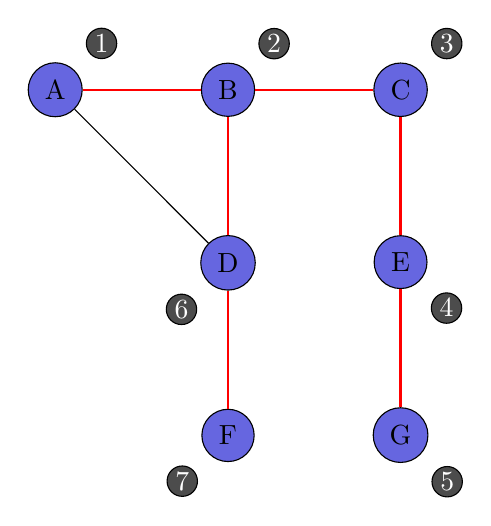
\begin{tikzpicture}[node distance=1.5cm, every node/.style={circle, draw, fill=blue!80!black!60}]
                \node (A) {A};
                \node (B) [right=of A] {B};
                \node (C) [right=of B] {C};
                \node (D) [below=of B] {D};
                \node (E) [below=of C] {E};
                \node (F) [below=of D] {F};
                \node (G) [below=of E] {G};

                \draw (A) -- (B);
                \draw (A) -- (D);
                \draw (B) -- (C);
                \draw (B) -- (D);
                \draw (C) -- (E);
                \draw (D) -- (F);
                \draw (E) -- (G);

                \foreach \i/\j in {A/B, B/C, C/E, E/G, B/D, D/F} {
                        \draw[thick, red] (\i) -- (\j);
                }

                % Add traversal order labels in white with dark gray circles
                \node[draw, circle, fill=black!70, inner sep=1pt] at (A) [above right=0.2cm and 0.2cm of A] {\textcolor{white}{1}};
                \node[draw, circle, fill=black!70, inner sep=1pt] at (B) [above right=0.2cm and 0.2cm of B] {\textcolor{white}{2}};
                \node[draw, circle, fill=black!70, inner sep=1pt] at (C) [above right=0.2cm and 0.2cm of C] {\textcolor{white}{3}};
                \node[draw, circle, fill=black!70, inner sep=1pt] at (D) [below left=0.2cm and 0.2cm of D] {\textcolor{white}{6}};
                \node[draw, circle, fill=black!70, inner sep=1pt] at (E) [below right=0.2cm and 0.2cm of E] {\textcolor{white}{4}};
                \node[draw, circle, fill=black!70, inner sep=1pt] at (F) [below left=0.2cm and 0.2cm of F] {\textcolor{white}{7}};
                \node[draw, circle, fill=black!70, inner sep=1pt] at (G) [below right=0.2cm and 0.2cm of G] {\textcolor{white}{5}};
        \end{tikzpicture}
\end{center}

\textbf{Cycle checking}: prune a path that ends in a node already on the path

DFS can be implemented recursively, with cycle checking.
With this implementation, the frontier is implicitly stored in the call stack.
\subsection{Properties of DFS}
\label{sec:org41f3308}
Properties:
\begin{itemize}
\item \emph{space complexity}: \(O(bm)\)
\item \emph{time complexity}: \(O(b^{m})\)
\item \emph{completeness}: no, will get stuck in infinite path (may or may not be cycle)
\item \emph{optimality}: no, pays no attention to cost
\end{itemize}

DFS is useful when:
\begin{itemize}
\item space is restricted
\item many solutions exist, possibly with long paths
\end{itemize}

DFS is poor when:
\begin{itemize}
\item infinite paths exist
\item optimal solutions are shallow
\item multiple paths to a node
\end{itemize}
\section{Breadth-First Search}
\label{sec:orgd6ccbd6}
Treats the frontier as a queue, select the earliest element added to the frontier to be expanded.

\begin{center}
        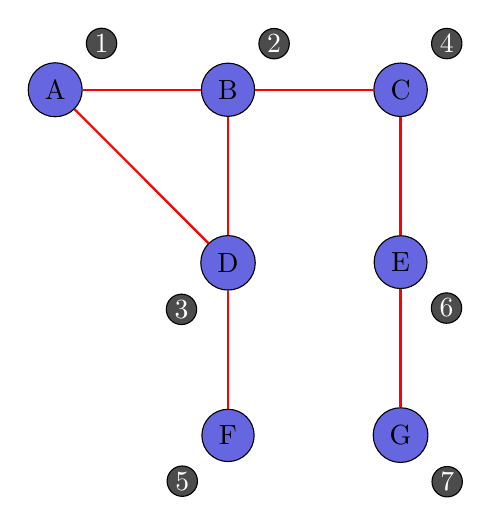
\begin{tikzpicture}[node distance=1.5cm, every node/.style={circle, draw, fill=blue!80!black!60}]
        \node (A) {A};
        \node (B) [right=of A] {B};
        \node (C) [right=of B] {C};
        \node (D) [below=of B] {D};
        \node (E) [below=of C] {E};
        \node (F) [below=of D] {F};
        \node (G) [below=of E] {G};

        \draw (A) -- (B);
        \draw (A) -- (D);
        \draw (B) -- (C);
        \draw (B) -- (D);
        \draw (C) -- (E);
        \draw (D) -- (F);
        \draw (E) -- (G);

        \foreach \i/\j in {A/B, A/D, B/C, B/D, C/E, D/F, E/G} {
                \draw[thick, red] (\i) -- (\j);
        }

        \node[draw, circle, fill=black!70, inner sep=1pt] at (A) [above right=0.2cm and 0.2cm of A] {\textcolor{white}{1}};
        \node[draw, circle, fill=black!70, inner sep=1pt] at (B) [above right=0.2cm and 0.2cm of B] {\textcolor{white}{2}};
        \node[draw, circle, fill=black!70, inner sep=1pt] at (D) [below left=0.2cm and 0.2cm of D] {\textcolor{white}{3}};
        \node[draw, circle, fill=black!70, inner sep=1pt] at (C) [above right=0.2cm and 0.2cm of C] {\textcolor{white}{4}};
        \node[draw, circle, fill=black!70, inner sep=1pt] at (F) [below left=0.2cm and 0.2cm of F] {\textcolor{white}{5}};
        \node[draw, circle, fill=black!70, inner sep=1pt] at (E) [below right=0.2cm and 0.2cm of E] {\textcolor{white}{6}};
        \node[draw, circle, fill=black!70, inner sep=1pt] at (G) [below right=0.2cm and 0.2cm of G] {\textcolor{white}{7}};
        \end{tikzpicture}
\end{center}
\subsection{Multi-Path Pruning}
\label{sec:orge603eba}
Prune a path to a given node than any path has been found to, since a path has already been found to it.

Pruning subsumes a cycle check, since the current path is a path to the node.

Requires storing all nodes paths have been found to, and must guarantee that this allows optimality.
\subsection{Properties of BFS}
\label{sec:org7366dae}
Properties:
\begin{itemize}
\item \emph{space complexity}: \(O(b^{d})\)
\item \emph{time complexity}: \(O(b^{d})\)
\item \emph{completeness}: yes, since it explores the tree level by level until it finds a goal
\item \emph{optimality}: no, it is guaranteed to find the shallowest goal node
\end{itemize}

BFS is useful when:
\begin{itemize}
\item space is no concern
\item a solution with the fewest arcs is desirable
\end{itemize}

BFS is a poor method when:
\begin{itemize}
\item all solutions are deep in the tree
\item problem is large and graph is dynamically generated
\end{itemize}
\section{Iterative Deepening Search}
\label{sec:org065ebf6}
For every depth limit, perform DFS until the depth limit is reached.

\begin{center}
    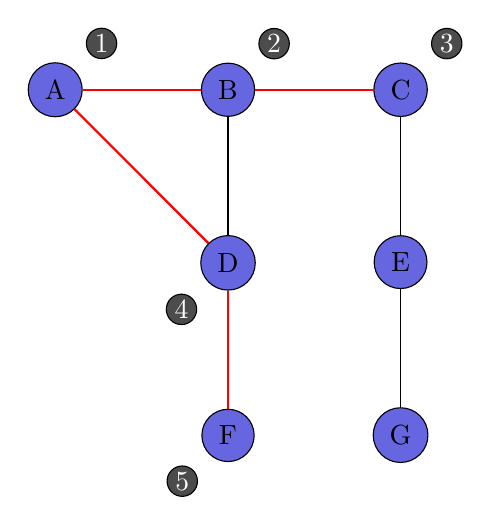
\begin{tikzpicture}[node distance=1.5cm, every node/.style={circle, draw, fill=blue!80!black!60}]
        % Nodes
        \node (A) {A};
        \node (B) [right=of A] {B};
        \node (C) [right=of B] {C};
        \node (D) [below=of B] {D};
        \node (E) [below=of C] {E};
        \node (F) [below=of D] {F};
        \node (G) [below=of E] {G};

        % Edges
        \draw (A) -- (B);
        \draw (A) -- (D);
        \draw (B) -- (C);
        \draw (B) -- (D);
        \draw (C) -- (E);
        \draw (D) -- (F);
        \draw (E) -- (G);

        % Highlighting the traversal order for depth 2
        \foreach \i/\j in {A/B, A/D, B/C, D/F} {
                \draw[thick, red] (\i) -- (\j);
        }

        % Traversal order numbers for depth 2
        \node[draw, circle, fill=black!70, inner sep=1pt] at (A) [above right=0.2cm and 0.2cm of A] {\textcolor{white}{1}};
        \node[draw, circle, fill=black!70, inner sep=1pt] at (B) [above right=0.2cm and 0.2cm of B] {\textcolor{white}{2}};
        \node[draw, circle, fill=black!70, inner sep=1pt] at (C) [above right=0.2cm and 0.2cm of C] {\textcolor{white}{3}};
        \node[draw, circle, fill=black!70, inner sep=1pt] at (D) [below left=0.2cm and 0.2cm of D] {\textcolor{white}{4}};
        \node[draw, circle, fill=black!70, inner sep=1pt] at (F) [below left=0.2cm and 0.2cm of F] {\textcolor{white}{5}};
        \end{tikzpicture}

    \vspace{1cm} % Space between the two graphs
        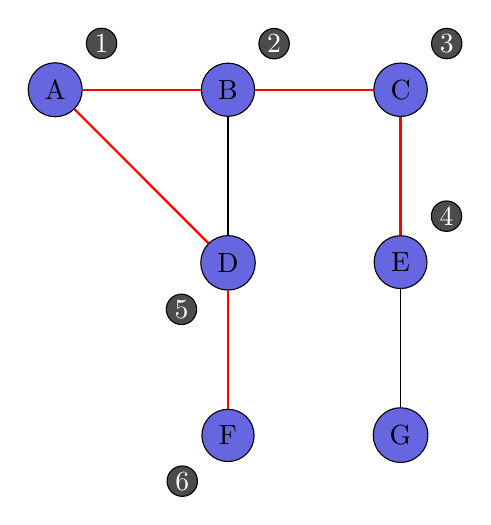
\begin{tikzpicture}[node distance=1.5cm, every node/.style={circle, draw, fill=blue!80!black!60}]
        % Nodes
        \node (A) {A};
        \node (B) [right=of A] {B};
        \node (C) [right=of B] {C};
        \node (D) [below=of B] {D};
        \node (E) [below=of C] {E};
        \node (F) [below=of D] {F};
        \node (G) [below=of E] {G};

        % Edges
        \draw (A) -- (B);
        \draw (A) -- (D);
        \draw (B) -- (C);
        \draw (B) -- (D);
        \draw (C) -- (E);
        \draw (D) -- (F);
        \draw (E) -- (G);

        % Highlighting the traversal order for depth 3
        \foreach \i/\j in {A/B, A/D, B/C, C/E, D/F} {
                \draw[thick, red] (\i) -- (\j);
        }

        % Traversal order numbers for depth 3
        \node[draw, circle, fill=black!70, inner sep=1pt] at (A) [above right=0.2cm and 0.2cm of A] {\textcolor{white}{1}};
        \node[draw, circle, fill=black!70, inner sep=1pt] at (B) [above right=0.2cm and 0.2cm of B] {\textcolor{white}{2}};
        \node[draw, circle, fill=black!70, inner sep=1pt] at (C) [above right=0.2cm and 0.2cm of C] {\textcolor{white}{3}};
        \node[draw, circle, fill=black!70, inner sep=1pt] at (E) [above right=0.2cm and 0.2cm of E] {\textcolor{white}{4}};
        \node[draw, circle, fill=black!70, inner sep=1pt] at (D) [below left=0.2cm and 0.2cm of D] {\textcolor{white}{5}};
        \node[draw, circle, fill=black!70, inner sep=1pt] at (F) [below left=0.2cm and 0.2cm of F] {\textcolor{white}{6}};
        \end{tikzpicture}
\end{center}
\subsection{Properties of IDS}
\label{sec:org3efc72c}
Properties:
\begin{itemize}
\item \emph{space complexity}: \(O(bd)\)
\item \emph{time complexity}: \(O(b^{d})\)
\item \emph{completeness}: yes, since it explores the tree level by level until it finds a goal
\item \emph{optimality}: no, it is guaranteed to find the shallowest goal node
\end{itemize}
\section{Lowest-Cost-First Search}
\label{sec:org6626f85}
Selects a path on the frontier with lowest cost, where the frontier is a priority queue ordered
by path cost.

It is an uninformed/blind search (does not take the goal into account).

\begin{center}
    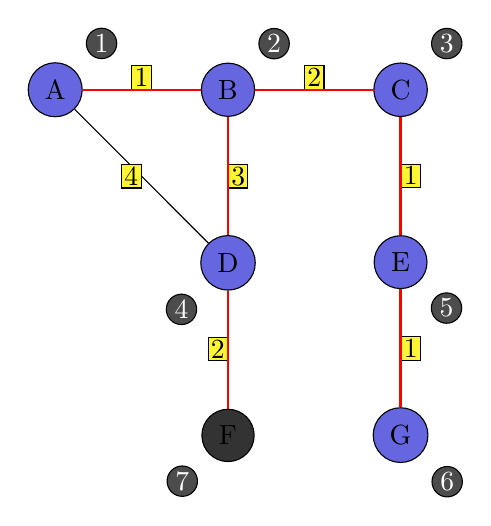
\begin{tikzpicture}[node distance=1.5cm, every node/.style={circle, draw, fill=blue!80!black!60}]
        \node (A) {A};
        \node (B) [right=of A] {B};
        \node (C) [right=of B] {C};
        \node (D) [below=of B] {D};
        \node (E) [below=of C] {E};
        \node (F) [below=of D, fill=black!80] {F}; % Goal node F highlighted
        \node (G) [below=of E] {G};

        \draw (A) -- (B);
        \draw (A) -- (D);
        \draw (B) -- (C);
        \draw (B) -- (D);
        \draw (C) -- (E);
        \draw (D) -- (F);
        \draw (E) -- (G);

        % Cost labels with better visibility
        \node[draw, rectangle, fill=yellow!80, text=black, inner sep=1pt] at ($(A)!0.5!(B)$) [above] {1};
        \node[draw, rectangle, fill=yellow!80, text=black, inner sep=1pt] at ($(A)!0.5!(D)$) [left] {4};
        \node[draw, rectangle, fill=yellow!80, text=black, inner sep=1pt] at ($(B)!0.5!(C)$) [above] {2};
        \node[draw, rectangle, fill=yellow!80, text=black, inner sep=1pt] at ($(B)!0.5!(D)$) [right] {3};
        \node[draw, rectangle, fill=yellow!80, text=black, inner sep=1pt] at ($(C)!0.5!(E)$) [right] {1};
        \node[draw, rectangle, fill=yellow!80, text=black, inner sep=1pt] at ($(D)!0.5!(F)$) [left] {2};
        \node[draw, rectangle, fill=yellow!80, text=black, inner sep=1pt] at ($(E)!0.5!(G)$) [right] {1};

        \foreach \i/\j in {A/B, B/C, B/D, C/E, D/F, E/G} {
            \draw[thick, red] (\i) -- (\j);
        }

        \node[draw, circle, fill=black!70, inner sep=1pt] at (A) [above right=0.2cm and 0.2cm of A] {\textcolor{white}{1}};
        \node[draw, circle, fill=black!70, inner sep=1pt] at (B) [above right=0.2cm and 0.2cm of B] {\textcolor{white}{2}};
        \node[draw, circle, fill=black!70, inner sep=1pt] at (D) [below left=0.2cm and 0.2cm of D] {\textcolor{white}{4}};
        \node[draw, circle, fill=black!70, inner sep=1pt] at (C) [above right=0.2cm and 0.2cm of C] {\textcolor{white}{3}};
        \node[draw, circle, fill=black!70, inner sep=1pt] at (F) [below left=0.2cm and 0.2cm of F] {\textcolor{white}{7}};
        \node[draw, circle, fill=black!70, inner sep=1pt] at (E) [below right=0.2cm and 0.2cm of E] {\textcolor{white}{5}};
        \node[draw, circle, fill=black!70, inner sep=1pt] at (G) [below right=0.2cm and 0.2cm of G] {\textcolor{white}{6}};
    \end{tikzpicture}
\end{center}
\subsection{Properties of LCFS}
\label{sec:orgcc2f058}
Properties:
\begin{itemize}
\item \emph{space complexity}: exponential
\item \emph{time complexity}: exponential
\item \emph{completeness}: yes
\item \emph{optimality}: yes
\end{itemize}

Completeness and optimality require that:
\begin{enumerate}
\item the branching factor is finite
\item the cost of every edge is strictly positive
\end{enumerate}
\subsection{Dijkstra's Algorithm}
\label{sec:org457a783}
Variant of LCFS with multi-path pruning.

Frontier is a PQ sorted by cost, with each node keeping track

\begin{center}
  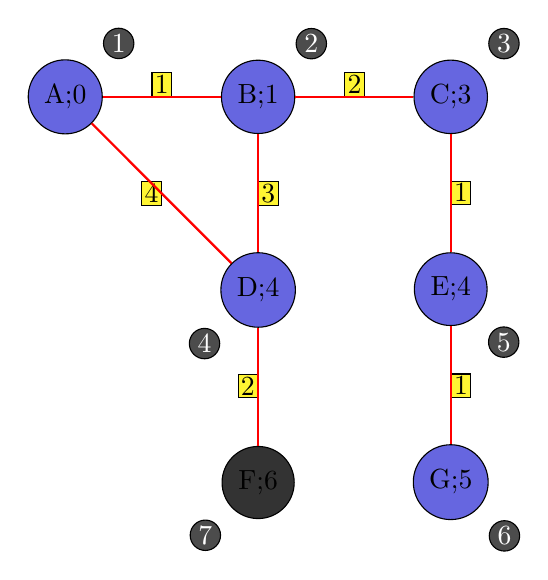
\begin{tikzpicture}[node distance=1.5cm, every node/.style={circle, draw, fill=blue!80!black!60}]
    \node (A) {A;0};
    \node (B) [right=of A] {B;1};
    \node (C) [right=of B] {C;3};
    \node (D) [below=of B] {D;4};
    \node (E) [below=of C] {E;4};
    \node (F) [below=of D, fill=black!80] {F;6}; % Goal node F highlighted
    \node (G) [below=of E] {G;5};

    \draw (A) -- (B);
    \draw (A) -- (D);
    \draw (B) -- (C);
    \draw (B) -- (D);
    \draw (C) -- (E);
    \draw (D) -- (F);
    \draw (E) -- (G);

    % Cost labels with better visibility
    \node[draw, rectangle, fill=yellow!80, text=black, inner sep=1pt] at ($(A)!0.5!(B)$) [above] {1};
    \node[draw, rectangle, fill=yellow!80, text=black, inner sep=1pt] at ($(A)!0.5!(D)$) [left] {4};
    \node[draw, rectangle, fill=yellow!80, text=black, inner sep=1pt] at ($(B)!0.5!(C)$) [above] {2};
    \node[draw, rectangle, fill=yellow!80, text=black, inner sep=1pt] at ($(B)!0.5!(D)$) [right] {3};
    \node[draw, rectangle, fill=yellow!80, text=black, inner sep=1pt] at ($(C)!0.5!(E)$) [right] {1};
    \node[draw, rectangle, fill=yellow!80, text=black, inner sep=1pt] at ($(D)!0.5!(F)$) [left] {2};
    \node[draw, rectangle, fill=yellow!80, text=black, inner sep=1pt] at ($(E)!0.5!(G)$) [right] {1};

    % Highlight the explored edges
    \foreach \i/\j in {A/B, A/D, B/C, B/D, C/E, D/F, E/G} {
        \draw[thick, red] (\i) -- (\j);
    }

    % Indicate traversal order with black circles
    \node[draw, circle, fill=black!70, inner sep=1pt] at (A) [above right=0.2cm and 0.2cm of A] {\textcolor{white}{1}};
    \node[draw, circle, fill=black!70, inner sep=1pt] at (B) [above right=0.2cm and 0.2cm of B] {\textcolor{white}{2}};
    \node[draw, circle, fill=black!70, inner sep=1pt] at (D) [below left=0.2cm and 0.2cm of D] {\textcolor{white}{4}};
    \node[draw, circle, fill=black!70, inner sep=1pt] at (C) [above right=0.2cm and 0.2cm of C] {\textcolor{white}{3}};
    \node[draw, circle, fill=black!70, inner sep=1pt] at (F) [below left=0.2cm and 0.2cm of F] {\textcolor{white}{7}};
    \node[draw, circle, fill=black!70, inner sep=1pt] at (E) [below right=0.2cm and 0.2cm of E] {\textcolor{white}{5}};
    \node[draw, circle, fill=black!70, inner sep=1pt] at (G) [below right=0.2cm and 0.2cm of G] {\textcolor{white}{6}};
\end{tikzpicture}
\end{center}
\end{document}
